\chapter{Consideraciones Especiales: Obstaculos y Soluciones} \label{chapter:consideraciones}

Durante el desarrollo del proyecto se presentaron algunos obstaculos que lograron ser resueltos. A continuación se describe la solución de algunos de esos obstáculos. 

Una de las primeras tareas ha sido configurar la tarjeta Arbotix para poder cargar programas en ella. Desde el IDE de Arduino, al intentar cargar un programa, se mostraban los siguientes errores:

"avrdude: stk500\_getsync(): not in sync: resp=0x3000"

"avrdude: stk500\_getsync(): not in sync: resp=0x00"

Uno de los problemas se debía a que, como el chip FTDI solo encajaba bien en un sentido, se estaba conectando de manera incorrecta. A través de ese chip se intentaba transmitir el código de la computadora a la Arbotix. La solución ha sido agregarle una extensión con cables, de tal forma de que se pudiera conectar en sentido contrario. 

Una vez solucionado este problema, los programas seguian sin poder cargarse. El siguiente problema era que no estaba guardado en la tarjeta Arbotix el gestor de arranque. Por lo cual se obtuvo el gestor 'Sanguino' y se cargó a la Arbotix a través del dispositivo programador para AVR llamado 'ISP programmer' que se muestra en la figura 

\begin{figure}[hbtp]
\centering
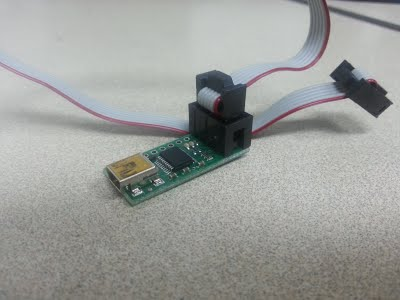
\includegraphics[scale=0.3]{imagenes/ISP.jpg}
\caption{Programador para AVR.}
\label{fig:trasera1}
\end{figure}

-----------


Quema de motores 

No teniamos monitor, TightVNC se utilizó para la visualización y control de la interfaz gráfica de Raspbian en la Raspberry Pi desde un computador remoto, pues es conveniente poder observar lo que el robot percibe para llevar un control y una supervisión de su comportamiento.

servidor de ROS version mala

Conectar bien el FTDI

Al principio no cargaban los programas a la arbotix, comprar isp y cargar bootloader
